\documentclass[12pt, letterpaper, twoside]{article}
\usepackage[utf8]{inputenc}
\usepackage{titlesec}
% Minted package is used for the command line samples provided in the document
\usepackage{minted}
\usepackage{graphicx}
\graphicspath{ {./} }

\newcommand{\sectionbreak}{\clearpage}

% removes the red box from the dollar sign that comes by default with minted.
\AtBeginEnvironment{minted}{\dontdofcolorbox}
\def\dontdofcolorbox{\renewcommand\fcolorbox[4][]{##4}}

\title{
    \textbf{Info-Mine}\\
    {Software lab project}\\
    {INDIAN INSTITUTE OF TECHNOLOGY, BOMBAY}
}
\author{ 
    \textbf{Rohit Kundu}\\203050030\\
    \textbf{Pranshu Chourasia}\\203050098\\
    \textbf{Raghunath Das}\\203050071\\
    \textbf{Pramod S Rao}\\20305R007\\
}

\date{18th November, 2020}

\begin{document}
\maketitle

\tableofcontents

\section{Introduction}
    The info-mine project aims at bringing together the information spread across various locations at IIT-B into one spot
    for a user to be able to access information faster and cleaner.

    \subsection{Motivation}
        Many of the courses tend to prefer certain platforms over the others for providing updates, quiz info, discussions etc. 
        Also, apart from the courses, we have two emails, which are insti and department.
        This causes a student to visit multiple sites many times which can get discomforting after a certain point, and students can also miss
        out on some updates.
        Thus, the aim of this project is to reduce the hindrance in visting many places and create a tool that helps students to get all their info
        in one spot. The term Info-Mine comes from mining for information from cse websites, moodle and the emails.
        
    \subsection{Installation}
    Write how to install here

\section{Moodle}
When using the moodle component of info-mine, they will have to provide their userid and password over command prompt.
A user will be prompted for these details only when using it for the first time and these details are encrypted and stored in the configs
folder. 
These credentials are then used to make the subsequent requests.
A user can then fetch 7 types of information from their moodle website, details of which are mentioned in the below subsections.
To find more info from the command line the user can simply perform the below command
\begin{minted}[frame=lines, framesep=4mm, encoding=utf8]{text}
/home/user$: python3 parser.py moodle -h
usage: parser.py moodle [-h] {quizzes,grades,forums,discussions,
courses,announcements,assignments} ...
positional arguments:
{quizzes,grades,forums,discussions,courses,announcements,assignments}
                        Moodle commands help
    quizzes             Info about quizzes
    grades              Info about grades
    forums              Info about discussion forums
    discussions         Info about discussions
    courses             Info about courses
    announcements       Info about announcements
    assignments         Info about assignments

optional arguments:
-h, --help            show this help message and exit

\end{minted}
    This provides the user with seven options from which he can choose to fetch his/her data.
    Let's start with quizzes.
\subsection{quizzes}
To get information on how to use the quizzes module, the user can do so with a -h flag like \\
\textbf{/home/user\$: python3 parser.py moodle quizzes -h}\\
\\
As you can see from the usage, by providing no flags, the user will simply get a list of all the quizzes for all the courses he/she has registered.\\
To get a list of the quizzes for a particular course, we need to use the -c flag with the course id(course id is with respect to moodle and can be found from the moodle courses module) we can for example:

\begin{minted}[frame=lines, framesep=4mm]{text}
/home/user$: python3 parser.py moodle quizzes -c 219

\end{minted}

\subsection{grades}
To get information on how to use the grades module, the user can do so with a -h flag like \\
\textbf{/home/user\$: python3 parser.py moodle grades -h}\\
\\
As you can see from the usage, by providing no flags, the user will simply get a list of all the grades for all the courses he/she has registered.\\
To get a list of the grades for a particular course, we need to use the -c flag with the course id(course id is with respect to moodle and can be found from the moodle courses module) we can for example:

\begin{minted}[frame=lines, framesep=4mm]{text}
/home/user$: python3 parser.py moodle grades -c 219
    
\end{minted}

\subsection{forums}
To get information on how to use the forums module, the user can do so with a -h flag like \\
\textbf{/home/user\$: python3 parser.py moodle forums -h}\\
\\
For using the forums module we need to provide -c flag and provide the course id (course id is with respect to moodle and can be found from the moodle courses module), it is mandatory. The -n flag is to provide the top number of entries we want to filter and see in the output\\
To get a list of 'n' forums for a course we can for example:

\begin{minted}[frame=lines, framesep=4mm]{text}
/home/user$: python3 parser.py moodle forums -c 219 -n 5
    
\end{minted}

\subsection{discussions}
To get information on how to use the discussions module, the user can do so with a -h flag like \\
\textbf{/home/user\$: python3 parser.py moodle discussions -h}\\
\\
For using the discussions module we need to provide -f flag and provide the forum id (forum id is with respect to moodle and can be found from the moodle forums module), it is mandatory to know which forum's discussion you are trying to fetch. The -n flag is to provide the top number of entries we want to filter and see in the output\\
To get a list of 'n' discussions for a forum we can for example:

\begin{minted}[frame=lines, framesep=4mm]{text}
/home/user$: python3 parser.py moodle discussions -f 219 -n 5
    
\end{minted}

\subsection{courses}
To get information on how to use the courses module, the user can do so with a -h flag like \\
\textbf{/home/user\$: python3 parser.py moodle courses -h}\\
\\
This is the simplest module to use as we don't have to pass any argument. We are simply returned a list of the courses in which we have registered.\\
Apart from courses registered, we also get important info like the course id which can be later used in the other moodle modules.
This also provides us with information on our progress made so far in the course.
Also, course code information is provided.
To get a list of courses we have registered:\\
\\
\begin{minted}[frame=lines, framesep=4mm]{text}
/home/user$: python3 parser.py moodle courses
sl No    Course id    Progress  Short Name     Full Name
-------  ----------- ----------  ------------- ----------
1  226   7.69231  CS 765-2020-1  Introduction to Blockchain
2  224   100      CS 744-2020-1  Design and Engineering of Computing Systems
3  219   88.8889  CS 699-2020-1  Software Lab.
\end{minted}

\subsection{announcements}
To get information on how to use the announcements module, the user can do so with a -h flag like \\
\textbf{/home/user\$: python3 parser.py moodle announcements -h}\\
\\
For using the announcements module we need to provide -c flag and provide the course id (course id is with respect to moodle and can be found from the moodle course module), it is mandatory to know which course's announcements you are trying to fetch. The -n flag is to provide the top number of entries we want to filter and see in the output\\
To get a list of 'n' announcements for a course we can for example:
\begin{minted}[frame=lines, framesep=4mm]{text}
/home/user$: python3 parser.py moodle discussions -c 226 -n 1
Announcements:
	 1. 2020-11-16 15:34:42 last lecture uploaded
Final lecture on Payment Channel Details has been uploaded (#26). 
Please see these before the Live Session on Thursday.Vinay
\end{minted}

\subsection{assignments}
To get information on how to use the assignments module, the user can do so with a -h flag like \\
\textbf{/home/user\$: python3 parser.py moodle assignments -h}\\
\\
For using the assignments module, the user needs to -c flag and provide the name of the course(or the substring of it). The -d flag filters out the due assignments. If no -c flag is provided it will list out all the assignments.\\
To get a list of the due assignments for a course we can for example:
\begin{minted}[frame=lines, framesep=4mm]{text}
/home/user$: python3 parser.py moodle assignments -c block -d
sl No  Course Name    Assignment    Due Date
-------  -------------  ------------  -------------------
      1  CS 765-2020-1  Assignment 2  2020-12-08 23:59:00
\end{minted}

\section{CSE}
The CSE component internally calls the cse website's APIs and fetches the required information. 
A user can fetch 4 types of information from the cse tool, details of which are mentioned in the below subsections.
A user can also find out more information by doing:
\begin{minted}[frame=lines, framesep=4mm, encoding=utf8]{text}
/home/user$: python3 parser.py cse -h
usage: parser.py cse [-h] {courses,students,faculties,news} ...

positional arguments:
  {courses,students,faculties,news}
                        CSE commands help
    courses             Info about courses
    students            Info about students
    faculties           Info about faculties
    news                Get news

optional arguments:
  -h, --help            show this help message and exit    
\end{minted}
This provides four options to fetch data from the cse website.
\subsection{courses}
The courses subcomponent can help us get the list of courses being offered for the year. It has filters for spring, autumn courses.
We can also fetch other information regarding a course such as it's description, the pre-requisites required for a course and it's text references.
To filter them out, we have the -f flag, we can filter them based on the course id, or course name or even the instructor name. This enables a user
with many options, For example, if a user wants to list out all the courses offered by professor 'X', user can do so using the appropriate flags
along with the -f flag.To get more info on the courses subcomponent, the user can do so using the -h flag\\
\textbf{/home/user\$: python3 parser.py cse courses -h}\\
\\
Some examples(Two examples):\\
To fetch all courses offered by Prof Kavi Arya along with description and text refs we can simply do:
\begin{minted}[frame=lines, framesep=4mm, encoding=utf8]{text}
/home/user$: python3 parser.py cse courses -f kavi -D -t
Course Name        Embedded Systems
Course Code        CS 684
Course Instructor  Prof. Kavi Arya
Semester           Spring
Description        Introduction to Embedded systems, hardware/software
                   codesign, 
                   Embedded micro controller cores, embedded memories, 
                   Examples of embedded systems, sensors and interfacing 
                   techniques, Real-time concepts, real-time operating 
                   systems, Required RTOS services/capabilities (in 
                   contrast with traditional OS).
                   Resource Management/scheduling paradigms: static 
                   priorities, static schedules, dynamic scheduling, 
                   best effort current best practice in scheduling 
                   (e.g. Rate Monotonic vs. static schedules), 
                   Real-world issues: blocking, unpredictability, 
                   interrupts, caching, 
                   Examples of OSs for embedded systems - RT Linux, VRTX.
                   Programming languages for embedded systems 
                   e.g., Handel-C and Esterel, system support for embedded 
                   systems, selected embedded system-based 
                   applications: process-control, robotics, etc. 
                   Software Development Methodology: Model based 
                   development, Statecharts, etc. Case studies, 
                   Controlling an Injection molding process, Flight simulator,
                   digital call center handler, codec.
References         Jack Ganssle, "The Art of Designing Embedded Systems", 
                   Newnes, 1999.
                   David Simon, "An Embedded Software Primer", 
                   Addison Wesley, 2000.
                   RTS: Real-Time Systems, by C.M. Krishna and Kang G. Shin, 
                   McGraw-Hill, 1997, ISBN 0-07-057043.
                   J. A. Stankovic and K. Ramamritham, Advances in Hard 
                   Real-Time Systems, IEEE Computer Society Press, 
                   Washington DC, September 1993, 
                   777 pages.Selected papers and references
....................................................
 
\end{minted}

Let's have a look at another example, where a user wants to know all the systems courses offered in spring, user can simply do:
\begin{minted}[frame=lines, framesep=4mm, encoding=utf8]{text}
/home/user$: python3 parser.py cse courses -f systems -s
Semester  Course Code    Course Name                                           
--------  -------------  --------------  
Spring   CS 317         Database and Information Systems                       
Spring   CS 347 M       Operating Systems                                      
Spring   CS 387         Database and Information Systems Lab                   
Spring   CS 681         Performance Analysis of Computer Systems and Networks  
Spring   CS 684         Embedded Systems
\end{minted}

\subsection{students}
This subcomponent helps us connect with other students of our batch. 
User can find information on other students such as their interests, advisors.
It has certain flags such as -b (to filter out the batchwise students), -i (to display their interests), -a (advisor)
and -f and -I to filter based on name and Interests respectively.
If we do not provide any options, the command will fetch all the students names from all the batches.\\
Using a mix and match of these flags, a user can fetch all types of information
that have been published in the cse website, this can help a user find information such as names of all students
under an advisor, names of all students with a specific interest and so on.\\
To get more info, the user can do using the -h flag:\\
\textbf{/home/user\$: python3 parser.py cse students -h}\\
\\
For example, to fetch the names of phd students who have an interest natural language processing
we can do so by:\\
\begin{minted}[frame=lines, framesep=4mm, encoding=utf8]{text}
/home/user$: python3 parser.py cse students -b phd -a -i -I natural
User ID     Name             Advisor                      
----------  ---------------  ---------------------------  
diptesh     Diptesh Kanojia  Prof. Pushpak Bhattacharyya  
kaverikale  Kaveri Kale                                   
\end{minted}

\subsection{faculties}
We can get all sorts of information on a faculty such as their room details, their website(if any),
a faculty's extension, interests. We can also filter faculties based on name
and interests. By providing no flags, it will simply return a list of all the faculties.
To find more info on how to use this, perform:\\
\textbf{/home/user\$: python3 parser.py cse faculties -h}\\
\\
Example where a user wants to fetch room information of faculties that 
have an interest in distributed systems. 
\begin{minted}[frame=lines, framesep=4mm, encoding=utf8]{text}
/home/user$: python3 parser.py cse faculties -I 'distributed systems' -r
User ID    Name                Room                                          
---------  ------------------  --------------------------------------------  
sri        Sridhar Iyer        Room no. SIA-420, Kanwal Rekhi Building       
rkj        Rushikesh K. Joshi  Room no. SIA-110, Kanwal Rekhi Building 
siva       G. Sivakumar        Room no. 508, 5th floor, New CSE/CC Building 
\end{minted}


\subsection{news}
This sub-component helps us find out the latest news posted on the cse website.
We can filter the news based on the timeline, a year and also get more details using the -t, -y and -d flags respectively.
For usage of this command, perform:\\
\textbf{/home/user\$: python3 parser.py cse news -h}\\
\\
To fetch news updates, in a certain timeline we can:
\begin{minted}[frame=lines, framesep=4mm, encoding=utf8]{text}
/home/user$: python3 parser.py cse news -t 16102020 17112020
Date        Snippet
----------  --------------------------------------------
2020-10-26  PhD students Ms. Durga Sivasubramanian and 
            Mr. Santhosh Kumar Guguloth have been selected 
            for the Prime Minister's Research Fellows (PMRF) Scheme

\end{minted}
\section{Mail}
Info-Mine, also consists of a component which helps us send and search for institure and department emails. We can do so using the command line with the appropriate flags. We can find the usage of the mail component by using the -h flag.\\
During the first time usage of this command, user credentials are asked, these credentials are encrypted and stored in the configs folder. These credentials are used for subsequent requests to send and receive mails.\\
\textbf{PLEASE NOTE: This component can send/search emails for both institute and department, the usage is the same for both, except that for department mail it is 'dmail' and for institute mail it is 'mail', this doc will show it only for mail.}\\
For usage of mail command, perform:\\
\textbf{/home/user\$: python3 parser.py mail -h}\\
\\
This gives out the options from which the user can send and search mails.
\subsection{Sending mail}
To send an email, a user has multiple options, such as -to for recepient, -sub for the subject, -b for body, -a for attachment, -fp for the local path of the attachment, -cc and -bcc for cc and bcc. For usage of this command: \\
\textbf{/home/user\$: python3 parser.py mail send -h}\\
\\
Example command to send an email with subject, body and attachment (Without cc and bcc):\\
\textbf{/home/user\$: python3 parser.py mail send -to "test@iitb.ac.in" -sub "test" -b "Test body" -a -fp "/root/path-to-file"}\\
Similarily, -cc and -bcc arguments can be provided to add cc and bcc recipients.

\subsection{Receiving mail}
To search for an email, a user has multiple options, such as -n to get the top n latest emails, -k to search for an email based on a keyword, -f to search based on from address, -s to search based on subject, -t to search based on the timeline.
For usage of search command in mail, perform:\\
\textbf{/home/user\$: python3 parser.py mail search -h}\\
\\
Example command to search top 2 latest emails :\\
\textbf{/home/user\$: python3 parser.py mail search -n 2}\\
\\
Example command to search top 2 latest emails between a specified timeline(The below command fetches the two latest emails between 10/11/20 and 15/11/20):\\
\textbf{/home/user\$: python3 parser.py mail search -n 2 -t 10112020 15112020}\\
\\
Example command to search top 2 latest emails with a specified subject (The string given will match substrings of the mail subjects):\\
\textbf{/home/user\$: python3 parser.py mail search -n 2 -s "power"}\\
\\
The other commands can be used in a similar way by the user to fetch the required mails.

\section{Whatsapp bot}

To use the Whatsapp bot, user will first need to register on the website.\\
http://infomine.pythonanywhere.com/ \\
Here you will have to provide all the details required and click the submit button. Once we have registered, the website will throw an alert which tells us to send a message to a whatsapp number and what message to send.\\
Number: +1 (415) 523-8886 \\
Initial Message: Join friend-identity \\
Doing this will create a channel of communication between the whatsapp bot and the user. \\
\textbf{In order to fetch information from the whatsapp bot, we have to perform the same commands as shown in sections 2, 3 and 4, without the "python3 parse.py"}\\
As seen in the image below: \\
\\
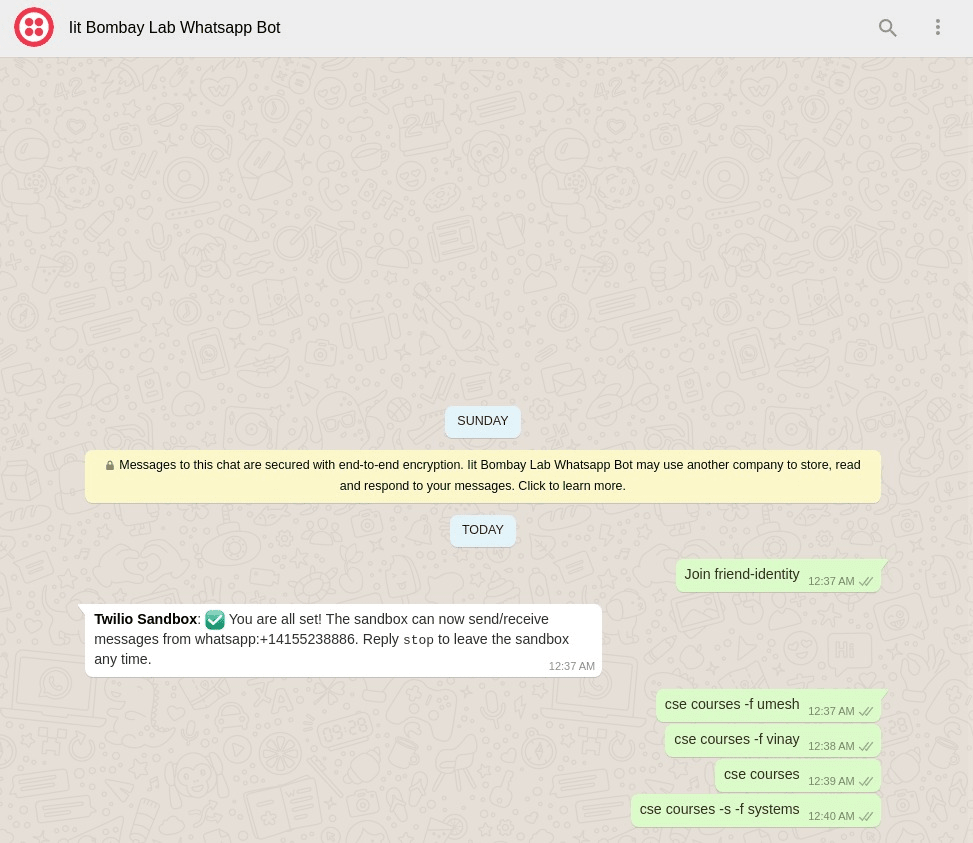
\includegraphics[width=14cm, height=10cm]{Latex_Image}

\section{Future scope}
This project aims at easing the life of a student at IIT-B by gathering most of the things in one place. A student can fetch information directly on command line when he or she is working on something, and does not have to use the UI and go through login procedures that you'd normally have to when fetching information otherwise.\\
The future improvements that can be made are to include fetching information from "Bodhitree", fetch updates from "Microsoft team APIs" and add features to the existing modules, such as getting a list of publications, information on exam timetable, academic timetable and so on.

\end{document}